% ---------------------------------------------------------------------
% EG author guidelines plus sample file for EG publication using LaTeX2e input
% D.Fellner, v1.17, Sep 23, 2010


\title[A Task Taxonomy to support Visualization for the Effective Analysis of Biological Pathways]%
      {A Task Taxonomy to support Visualization for the Effective Analysis of Biological Pathways}

% for anonymous conference submission please enter your SUBMISSION ID
% instead of the author's name (and leave the affiliation blank) !!
\author[]{SUBMISSION ID}

% ------------------------------------------------------------------------

% if the Editors-in-Chief have given you the data, you may uncomment
% the following five lines and insert it here
%
% \volume{27}   % the volume in which the issue will be published;
% \issue{1}     % the issue number of the publication
% \pStartPage{1}      % set starting page


%-------------------------------------------------------------------------
\begin{document}

% \teaser{
%  
\includegraphics[width=\linewidth]{eg_new}
%  \centering
%   \caption{New EG Logo}
% \label{fig:teaser}
% }

\maketitle

\begin{abstract}
Understanding complicated networks of interactions and chemical components is essential to solving contemporary problems in modern biology, especially in domains such as cancer and systems research.
In these domains, biological pathway data is used to represent chains of interactions that occur within a given biological process.
Visual representations can help researchers understand and interact with complex pathway data in a number of ways. 
Biological data sets offer unique challenges for visualization, due to their complexity and heterogeneity.

Here, we present taxonomy of tasks that are regularly performed by researchers who work with biological pathway data. 
These tasks were generated from interviews with several domain experts and require further classification than is provided by existing taxonomies. 
We also examine the existing visualization techniques which support each of the tasks, and we discuss gaps in the existing visualization space revealed by our taxonomy. 
We conclude by suggesting future research directions based on our taxonomy and motivated by the comments received by our domain experts.


\begin{classification} % according to http://www.acm.org/class/1998/
\CCScat{Computer Graphics}{I.3.3}{Picture/Image Generation}{Line and curve generation}
\end{classification}

\end{abstract}

%-------------------------------------------------------------------------
\section{Introduction}

Understanding complicated networks of interactions and chemical components is essential to solving contemporary problems in modern biology, especially in domains such as cancer and systems research~\cite{hanahan2011hallmarks}. 
In order to limit the scope of their analyses, researchers often work with \emph{pathways}, which are used to describe a chain of interactions between biochemical and biological entities within a cell.
Pathways are small, curated subsets of a much larger, complex graph of interactions between molecules, and a given pathway usually represents a particular biological process that is relevant within some research context.
 For example, Figure \ref{fig:kvik} shows a typical representation of a pathway as a human-curated node-link diagram, where nodes are biological entities and edges represent interactions between them.

\begin{figure}[htb]
  \centering
  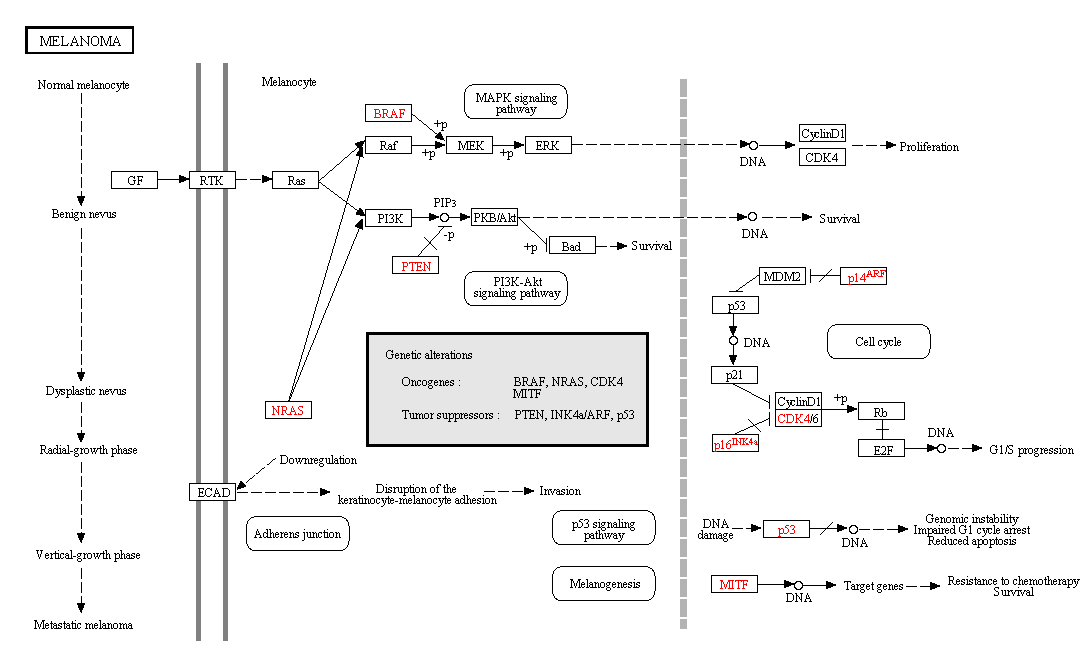
\includegraphics[width=\linewidth]{figures/kegg2}
  \caption{\label{fig:kvik} A view of a typical KEGG diagram. From~\cite{Fjukstad2014kvik}.}
\end{figure}

%\p{Pathways are very complex}

Researchers who work with pathway data are confronted with a number of challenges.
Pathway files may contain hundreds of proteins and biomolecules that participate in a variety of reactions.
In an abstract sense, reactions can be seen as state transitions with multiple inputs and outputs.
Participants --- genes, proteins, and other molecules within a cell --- can act as inputs or outputs to multiple reactions, and the relationships between reactions inherently include feedback loops.
Reactions often have an effect on other reactions, inhibiting or promoting their frequency.
These molecular activation pathways are inherently dynamic, which limits the utility of any static graph representation \cite{kitano2002systems}.
Representing complexity while also enabling researchers to see higher order patterns is a significant challenge \cite{saraiya2005visualizing}.

%\p{Pathways are useful for presentation}

Pathway diagrams can be useful for both presentation and analysis.
For presentation, pathway diagrams can contextualize a set of biological processes within a cell, and diagrams often show the location of cellular membranes in order to help provide a frame of reference for a given process.
Ideally, a pathway diagram allows a viewer to efficiently understand a complex set of biological relationships.

%\p{Pathways are useful for analysis}

While pathways may be useful for presenting and contextualizing a set of reactions, they can also be an important part of analyses in domains related to molecular biology and systems research, among others.
%\p{Domain context}

For example, molecular activation pathways are of critical importance to cancer researchers, who hope to understand --- and potentially disrupt --- malignant cycles of uncontrolled cellular growth, replication, and mediated cell death \cite{cairns2011regulation}.
Effective cancer drug development involves determining how proteins affected by a drug in turn affect important cellular pathways, and in this domain the downstream consequences of a particular drug effect are especially important \cite{luo2003targeting}.
In a separate domain, stem-cell researchers work with pathways that will precipitate a desired cellular differentiation into specific cell types \cite{reya2001stem}.

%\p{Static representations are not enough}

In the last decade, analyses that involve hundreds or thousands of genes and gene products have become common. When analyzing such large and complex data, visual representations can be essential.
Often, static representations are inadequate.
The complexity and amount of information that needs to be incorporated in given diagram can make static representations cluttered and difficult to interpret.
Thus, modern tools make careful use of user interactions and visualization techniques to allow a user to effectively explore and analyze pathway data.

%\p{Designing effective tools}

Designing effective visual analytics applications requires a detailed understanding of analysis tasks that are performed by the user.
Pathway data are often large and complex, and analysts will want to perform a variety of tasks depending on their research domain.
Tasks may be exploratory in nature, and a useful visualization of pathway data could reveal new insights to a researcher.
Tasks may also involve detailed queries or calculations of various network metrics, for example.
A comprehensive understanding of tasks performed by domain researchers in a typical analysis is essential to the design and implementation of an effective visual analytics application.

%\p{Other reviews}

Here we perform a comprehensive analysis of tasks and requirements in an effort to design effective platforms for visual analytics of pathway data.
Previous reviews of pathway analysis tools~\cite{Gehlenborg2010omics,Suderman2007tools} have surveyed the population of available applications.
However, the most recent review was published over five years ago, and it includes only a surface-level discussion of tasks, requirements, and visual encoding techniques.

%\p{In this work}

In this work, we present a description and analysis of tasks and requirements related to biological pathway research.
Tasks were gathered from several interviews with domain experts who work with biological pathway data.
After an introduction to the structure and content of pathway data, we describe the tasks that were garnered from our interviews.
Using these tasks, we then describe the high-level requirements of an effective visual analytics platform for pathway data.
We then review visual representations of pathway data in the context of our requirements.
We also review existing tools that implement those visual representations.
Finally, avenues of future research are considered, along with a brief summary of lessons learned from domain experts.

\subsection{Pathway data}

In order to aid an understanding of pathway visualization tools, an understanding of the structure of pathway data structures is necessary.
In this section we briefly explain the structure of typical pathway data files. 

\subsubsection{Pathway Data Model}

Information stored in any pathway data file can generally be broken down into three components:

\begin{itemize}

\item \textbf{Entity}\\
An entity is a component of a pathway such as a gene, a gene product (i.e. a protein), a complex of proteins, or a small biomolecule within a cell.
Entities are identified by name and are involved in one or more relationships.
Importantly, pathways themselves can be entities within other pathways.
\item \textbf{Relationship}\\
A relationship involves two or more entities.
Various kinds of relationships which different biological meanings are present in a pathways.
Relationships can be directed or undirected, and they can involve more than two entities.
\item \textbf{Meta-data}\\
The complex nature of the information stored in a pathway requires additional data to be stored with each entity and relationship.
Meta-data can include experimental data, scientific information such as the molecular structure of a chemical compound, as well as links to additional resources or publications related to an entity or relationship.

\end{itemize}


\subsubsection{Pathway Data Formats}

Pathway data can be stored in one of several file formats.
In particular \textit{BioPAX}~\cite{demir2010biopax}, \textit{KEGG}~\cite{kanehisa2000kegg} and \textit{SBML} are the most popular standards for storing the complex data structure described in the previous section.
These formats are XML based and represent data as an ontology. 
\emph{BioPAX}, in particular, was designed to be a general format for biological pathways across a variety of domain contexts~\cite{demir2010biopax}.

Other formats are employed for the visualization of biological pathways that are not specific to the field of biology.
For instance \textit{SIF Simple Interaction Format} used by \textit{Cytoscape}~\cite{Shannon2003cytoscape} is used to visualize undirected interactions between participants.
%-------------------------------------------------------------------------
\section{Instructions}

%-------------------------------------------------------------------------
\subsection{Language}

%-------------------------------------------------------------------------
\subsection{Margins and page numbering}


%------------------------------------------------------------------------
\subsection{Formatting your paper}

%-------------------------------------------------------------------------
\subsection{Type-style and fonts}


%-------------------------------------------------------------------------
\subsection{Illustrations, graphs, and photographs}

All graphics should be centered.


%-------------------------------------------------------------------------

%\bibliographystyle{eg-alpha}
\bibliographystyle{eg-alpha-doi}

\bibliography{references}


\end{document}
